\documentclass[
  digital,     %% The `digital` option enables the default options for the
               %% digital version of a document. Replace with `printed`
               %% to enable the default options for the printed version
               %% of a document.
%%  color,       %% Uncomment these lines (by removing the %% at the
%%               %% beginning) to use color in the printed version of your
%%               %% document
  oneside,     %% The `oneside` option enables one-sided typesetting,
               %% which is preferred if you are only going to submit a
               %% digital version of your thesis. Replace with `twoside`
               %% for double-sided typesetting if you are planning to
               %% also print your thesis. For double-sided typesetting,
               %% use at least 120 g/m² paper to prevent show-through.
  nosansbold,  %% The `nosansbold` option prevents the use of the
               %% sans-serif type face for bold text. Replace with
               %% `sansbold` to use sans-serif type face for bold text.
  nocolorbold, %% The `nocolorbold` option disables the usage of the
               %% blue color for bold text, instead using black. Replace
               %% with `colorbold` to use blue for bold text.
  lof,         %% The `lof` option prints the List of Figures. Replace
               %% with `nolof` to hide the List of Figures.
  lot,         %% The `lot` option prints the List of Tables. Replace
               %% with `nolot` to hide the List of Tables.
]{fithesis4}
%% The following section sets up the locales used in the thesis.
\usepackage[resetfonts]{cmap} %% We need to load the T2A font encoding
\usepackage[
  main=english, %% By using `czech` or `slovak` as the main locale
                %% instead of `english`, you can typeset the thesis
                %% in either Czech or Slovak, respectively.
  % english, german, russian, czech, slovak %% The additional keys allow
]{babel}        %% foreign texts to be typeset as follows:
%%
%%   \begin{otherlanguage}{german}  ... \end{otherlanguage}
%%   \begin{otherlanguage}{russian} ... \end{otherlanguage}
%%   \begin{otherlanguage}{czech}   ... \end{otherlanguage}
%%   \begin{otherlanguage}{slovak}  ... \end{otherlanguage}
%%
%% For non-Latin scripts, it may be necessary to load additional
%% fonts:
\usepackage{paratype}
% \def\textrussian#1{{\usefont{T2A}{PTSerif-TLF}{m}{rm}#1}}
%%
%% The following section sets up the metadata of the thesis.
\thesissetup{
    date        = \the\year/\the\month/\the\day,
    university  = mu,
    faculty     = fi,
    type        = bc,
    department  = Department of Computer Systems and Communications,
    author      = Dominik Tichý,
    gender      = m,
    advisor     = {RNDr. Tomáš Raček, Ph.D.},
    title       = {Modern visualization of partial atomic charges in Mol*},
    TeXtitle    = {Modern visualization of partial atomic charges in Mol*},
    keywords    = {%
        Mol*,
        ACC~II,
        αCharges,
        AlphaFold,
        SB NCBR,
        molecular visualization,
        molecular structures,
        partial atomic charges,
        structural biology,
        chemical file formats
    },
    TeXkeywords = {%
        Mol*,
        ACC~II,
        αCharges,
        AlphaFold,
        SB NCBR,
        molecular visualization,
        molecular structures,
        partial atomic charges,
        structural biology,
        chemical file formats
    },
    abstract    = {%
        TODO
    },
    thanks      = {%
        TODO
    },
    bib         = {%
        main.bib,
    },
    %% Remove the following line to use the JVS 2018 faculty logo.
    facultyLogo = fithesis-fi,
}
\usepackage{tipa}
\usepackage{makeidx}      %% The `makeidx` package contains
\makeindex                %% helper commands for index typesetting.
%% These additional packages are used within the document:
\usepackage{paralist} %% Compact list environments
\usepackage{amsmath}  %% Mathematics
\usepackage{amsthm}
\usepackage{amsfonts}
\usepackage{url}      %% Hyperlinks
\usepackage{markdown} %% Lightweight markup
\usepackage{listings} %% Source code highlighting
\lstset{
  basicstyle      = \ttfamily,
  identifierstyle = \color{black},
  keywordstyle    = \color{blue},
  keywordstyle    = {[2]\color{cyan}},
  keywordstyle    = {[3]\color{olive}},
  stringstyle     = \color{teal},
  commentstyle    = \itshape\color{magenta},
  breaklines      = true,
}
\usepackage{floatrow} %% Putting captions above tables
\floatsetup[table]{capposition=top}
\usepackage[babel]{csquotes} %% Context-sensitive quotation marks
\usepackage{minted}
\usepackage{subfigure}
\usepackage{textalpha}
\usepackage{dirtree}
\usepackage[export]{adjustbox}
\usepackage{pdfpages}
\usepackage{chemfig}
\usepackage{listings}

\begin{document}

\newpage
\chapter*{Introduction}
\markright{\textsc{Introduction}}
\addcontentsline{toc}{chapter}{Introduction}

Partial atomic charges are real numbers that describe a molecule's electron density. They are used in various fields of computational chemistry, such as molecular dynamics, molecular docking, and pharmacophore design. \cite{racek2022thesis} While partial atomic charges cannot be directly measured experimentally, they can be calculated using computational methods based on quantum mechanics. \cite{gupta2015principles} However, these methods pose significant computational challenges, particularly for larger molecules, leading researchers to employ faster, albeit less accurate, empirical methods. \cite{schindler2019thesis}

Atomic Charge Calculator II \cite{racek2020acc2} and αCharges \cite{schindler2023alphacharges} are two web-based applications that allow rapid calculations of partial atomic charges by empirical methods. The Atomic Charge Calculator II application incorporates the Litemol viewer \cite{sehnal2017litemol} to enable users to visualize the calculated charges. However, the Litemol viewer is no longer maintained, and its replacement, the Mol* viewer \cite{sehnal2021molstar}, does not currently support the visualization of partial atomic charges.

The absence of this functionality in the Mol* viewer presents a significant limitation for researchers in computational chemistry. Therefore, this thesis aims to address this limitation by extending the Mol* viewer to support the visualization of partial atomic charges and, subsequently, incorporating the enhanced Mol* viewer into the Atomic Charge Calculator II and αCharges web applications.

Chapter \ref{chapter:theory} introduces the theoretical concepts of molecular structures and partial atomic charges, along with the chemical file formats utilized in this work. Building on this foundation, Chapter \ref{chapter:visualizing_molecular_data} discusses the various visualization methods and software tools for visualizing molecular structures. Chapter \ref{chapter:molstar_partial_charges_extension} then describes the implementation of the Mol* viewer extension for visualizing partial atomic charges. Finally, the extended Mol* viewer is integrated into the Atomic Charge Calculator II and αCharges web applications, as detailed in Chapters \ref{chapter:atomic_charge_calculator_ii} and \ref{chapter:alphacharges}.

Through these efforts, this thesis seeks to advance the field of computational chemistry by providing researchers with a modern visualization of partial atomic charges in Mol*.

\newpage
\chapter{Theory}
\label{chapter:theory}

Theoretical concepts are fundamental to the study of computational chemistry, providing a framework for analyzing molecular structures and properties. This chapter focuses on four key areas of theory, beginning with an overview of molecular structures in Section 1.1. Section 1.2 explores partial atomic charges
examination of chemical file formats, including the advantages and disadvantages of different file formats for storing molecular data. Partial atomic charges are explored in section 1.3, including their importance in analyzing molecular structures and the various methods used to compute them. Finally, section 1.4 describes color interpolation, a critical technique for visualizing partial atomic charges in molecular structures.

By providing a comprehensive overview of these theoretical concepts, this chapter provides a strong foundation for the subsequent chapters, focusing on the implementation and analysis of the Mol* extension for visualizing partial atomic charges in molecular structures.

\section{Molecular structure}
\label{section:molecular_structure}

% TODO: the section is not split into many subsections to allow for better reading flow; first i describe small molecules (micromolecules) which are just described by their atoms and bonds, these are usually drug molecules (think ligands, ions etc); for macromolecules explain the hierarchy of chain-residue-atom, in this work we used carbohydrates and proteins - describe those as well; explain somehow that this separation is done on purpose; add a schematic image that shows a small protein with 2 chains, then zoom in on one chain and show the residues, lastly zoom on one of the residues to show the atoms and bonds \\

% TODO: don't focus too much on explaining things that aren't relevant further in the thesis \\

Molecules are the fundamental building blocks of matter, consisting of two or more atoms connected by chemical bonds. Molecules can vary widely in size and complexity, ranging from simple diatomic molecules like oxygen (O2) to highly complex organic compounds like proteins and DNA
Molecules are composed of atoms, which are connected through chemical bonds. Molecules can be divided into two main categories: micromolecules and macromolecules.

In this thesis work, we focus on two types of molecules: micromolecules and macromolecules. Micromolecules are relatively small in size and typically consist of a limited number of atoms. They are characterized by their low molecular weight and simple structure. Micromolecules play crucial roles in various biological processes and are involved in numerous chemical reactions in living organisms. Examples of micromolecules include water, glucose, or ethanol.

The reason for this separation is that micromolecules are usually drug molecules (think ligands, ions, etc.), while macromolecules are usually proteins or carbohydrates. The structure of micromolecules is typically represented by their constituent atoms and bonds. The atoms are represented by their chemical symbols, while the bonds are represented by lines connecting the atoms. The atoms and bonds are arranged in a two-dimensional (2D) or three-dimensional (3D) space, depending on the molecule's structure. Figure \ref{fig:micromolecule} shows the 2D structure of ethanol, a micromolecule consisting of two carbon atoms, six hydrogen atoms, and one oxygen atom. 

\subsection{Micromolecules}

Micromolecules, also known as small molecules, are relatively small in size and typically consist of a limited number of atoms. They are characterized by their low molecular weight and simple structure. Micromolecules play crucial roles in various biological processes and are involved in numerous chemical reactions in living organisms. Examples of micromolecules include water, glucose, or ethanol.

The structure of micromolecules is typically represented by their constituent atoms and bonds. The atoms are represented by their chemical symbols, while the bonds are represented by lines connecting the atoms. The atoms and bonds are arranged in a two-dimensional (2D) or three-dimensional (3D) space, depending on the molecule's structure. Figure \ref{fig:micromolecule} shows the 2D structure of ethanol, a micromolecule consisting of two carbon atoms, six hydrogen atoms, and one oxygen atom.

% \begin{figure}[htbp]
%   \centering
%   \chemfig{-[2]H(-[6]H)-C(-[2]H)(-[6]H)-O-H}
%   \caption{Hierarchy of structure 1A1U.}
%   \label{fig:micromolecule}
% \end{figure}


Micromolecules are small molecules typically consisting of a relatively low number of atoms.

Micromolecules are involved in various cellular processes and perform essential functions within living organisms.

Examples of micromolecules include:

\subsection{Macromolecules}

Macromolecules are large molecules composed of a high number of atoms, often thousands or even millions.

They are typically formed through polymerization, where smaller subunits, called monomers, combine to form larger chain-like structures. This structure of macromolecules is hierarchical, consisting of chains, residues, and atoms.

 Macromolecules are crucial for the structure, function, and regulation of cells and organisms. Their large size allows for complex interactions and the ability to carry out specialized tasks within living systems.

There are four major classes of biological macromolecules: proteins, nucleic acids, carbohydrates, and lipids.

Proteins are composed of amino acid monomers, proteins play crucial roles in cell structure, enzyme catalysis, immune response, and cell signaling.

Nucleic Acids: DNA (deoxyribonucleic acid) and RNA (ribonucleic acid) are nucleic acids, which are polymers of nucleotide monomers. They store and transmit genetic information and are involved in protein synthesis.

Carbohydrates are composed of sugar monomers, carbohydrates include simple sugars (monosaccharides), double sugars (disaccharides), and complex carbohydrates (polysaccharides). They provide energy and serve as structural components in cells.

Lipids are a diverse group of molecules that include fats, oils, phospholipids, and steroids. Lipids are hydrophobic and serve as energy storage, insulation, and structural components of cell membranes.


A residue refers to a specific monomer or building block within a macromolecule. In the case of proteins, each residue corresponds to an amino acid. For nucleic acids, each residue corresponds to a nucleotide. Residues are linked together by chemical bonds to form chains.

A chain is a linear sequence of residues within a macromolecule. It represents the backbone of the molecule, with each residue connected to the next one. In proteins, the chain is often referred to as a polypeptide chain.

% Alternative conformations, also referred to as conformational isomerism, are different conformations of the same molecule. They can be used to represent different states of a molecule, such as different protonation states or different ligand binding modes. Alternative conformations are important for understanding the structure and function of biomolecules, as they provide insight into how they interact with other molecules.

\begin{figure}[htbp]
  \centering
  \subfigure[Residues of chain B.]{\label{fig:structure1}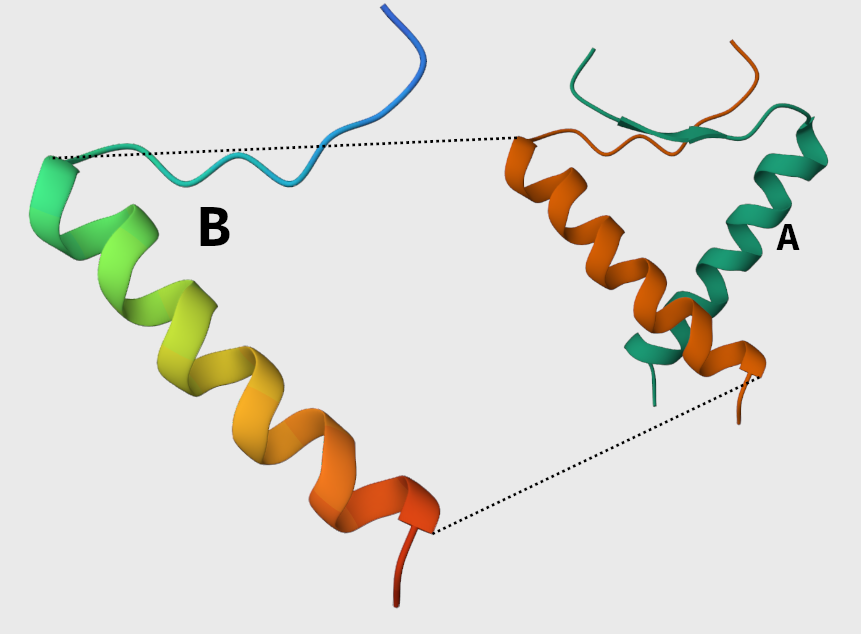
\includegraphics[height=4.5cm]{figures/structure1.png}}
  \subfigure[Atoms of residue ARG 19.]{\label{fig:structure2}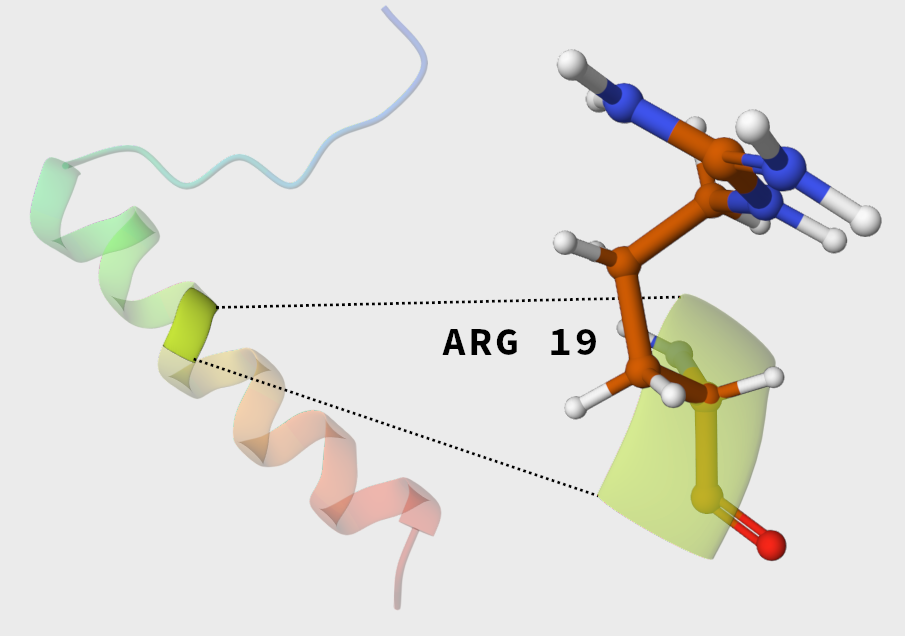
\includegraphics[height=4.5cm,]{figures/structure2.png}}
  \caption{Hierarchy of structure 1A1U.}
  \label{fig:structure}
\end{figure}


\section{Partial atomic charges}
\label{section:partial_atomic_charges}

When two atoms of a molecule form a chemical bond, they share electrons. However, the electrons are not evenly shared between the two atoms due to differences in their electronegativities \footnote[1]{Electronegativity is a measure of an atom's ability to attract electrons towards itself. \cite{racek2022thesis}}. Atoms with higher electronegativities attract electrons more strongly than atoms with lower electronegativities. This uneven distribution of electron density influences the physical properties of the molecule and determines how it interacts with other molecules or substances.One way to represent this uneven distribution of electron density is by assigning partial atomic charges to individual atoms within the molecule. 

Partial atomic charges are numerical values assigned to individual atoms within a molecule, representing their contribution to the distribution of electron density. Atoms with higher electronegativities have a partial negative charge, while atoms with lower electronegativities have a partial positive charge. Figure \ref{fig:partial_atomic_charges} shows the partial atomic charges of water (H2O). The partial atomic charges are represented by the red and blue spheres, with the red spheres representing the partial negative charges and the blue spheres representing the partial positive charges. 

There are several applications for partial atomic charges in computational chemistry, such as molecular dynamics, molecular docking, and pharmacophore design. \cite{racek2022thesis}

% TODO: maybe break it up here into a subsection about calculation methods

It is important to note that partial charges are simplify a theoretical concept and cannot be directly measured or observed; they can only be calculated using computational methods. One approach for calculating partial atomic charges is by quantum mechanical methods. However, these methods are computationally expensive and require a lot of computational resources. Another approach is by empirical methods, which are less accurate but faster and more efficient than quantum mechanical methods. \cite{schindler2019thesis}

Empirical methods are an efficient alternative to quantum mechanical methods, which operate at the atomic level rather than directly considering individual electrons or molecular orbitals. These methods aim to produce charges that are comparable to those obtained through quantum mechanical methods while keeping the computational complexity manageable. \cite{racek2022thesis}

There are several empirical methods for calculating partial atomic charges, such as the EEM (Electronegativity Equalization Method), SQE+qp (Semi-Quantitative Electrostatic Potential Method), and MMFF (Merck Molecular Force Field). These methods are based on the assumption that the electron density of a molecule can be approximated by a sum of atomic densities. \cite{racek2022thesis}

\section{Chemical file formats}
\label{section:chemical_file_formats}

Chemical file formats are used to store molecular data in a computer-readable format. There are several file formats for storing molecular data, each suited to a specific purpose. This section provides an overview of the most common file formats used in computational chemistry: SDF, MOL2, PDB, and mmCIF.

\subsection{SDF}
\label{subsection:sdf}

Structure-data file (SDF) is a widely used text-based chemical file format for describing the atoms, bonds, and atomic coordinates of small molecules. It is a container for the MOL V2000 and V3000 file formats. The SDF format is commonly used in cheminformatics applications, such as molecular modeling and drug discovery.

Figure \ref{} depicts the contents of an SDF file containing the structure of phenol in the MOL V2000 format.

% The first line contains the name of the molecule, followed by the number of atoms and bonds in the molecule. The next lines contain the atomic coordinates of each atom, followed by the bond information.

\begin{figure}[htbp]
  \centering
  \lstset{
    basicstyle=\ttfamily,
    breaklines=true,
    columns=fullflexible
    }
    \lstinputlisting[firstline=1, lastline=10]{phenols.sdf}
    \caption{First ten lines of a SDF file containing the structure of a phenol.}
    \label{fig:sdf}
  \end{figure}

\subsection{MOL2}
\label{subsection:mol2}

The Mol2 file format is another text-based format for storing small molecular structures and their associated properties. It can store multiple conformations of a molecule and is commonly used in molecular modeling and cheminformatics applications. The Mol2 format provides more flexibility and additional features compared to the SDF format, such as support for multiple substructures and atom types.

\begin{figure}[htbp]
  \centering
  \lstset{
    basicstyle=\ttfamily,
    breaklines=true,
    columns=fullflexible
    }
    \lstinputlisting[firstline=1, lastline=10]{phenols.mol2}
    \caption{First ten lines of a MOL2 file containing the structure of a phenol.}
    \label{fig:mol2}
  \end{figure}


\subsection{PDB}
\label{subsection:pdb}

\cite{gu2009structural}

The Protein Data Bank (PDB) file format is a widely used format for storing three-dimensional structures of proteins, nucleic acids, and other macromolecules. PDB files contain information about the atomic coordinates, secondary structure, and other important details required for understanding macromolecular structures. The PDB format has been widely adopted in structural biology, bioinformatics, and related fields.

\subsection{mmCIF}
\label{subsection:mmcif}

% TODO: explain the need for creating the mmCIF file format, why isn't the PDB format enough (limited amount of rows, poor support for extending the format to add custom data)? describe the mmcif file format; make sure to explain the core data dictionaries, can mention binary cif \\

\cite{gu2009structural}

The macromolecular Crystallographic Information File (mmCIF) format is an extension of the CIF format, specifically designed for macromolecular structures.
It is a text-based format that provides a more comprehensive and flexible representation of macromolecular crystallography data compared to the PDB format.
One of the most important features of the mmCIF format is its support for data dictionaries.
This allows users to define new data items and integrate additional information.
In contrast to other formats, the mmCIF format does not impose limits on column width and entry count, making it more flexible and accommodating for storing large amounts of data.

% TODO: add example image + better explanation

% \section{Color interpolation}
% \label{section:color_interpolation}

% % TODO: this section will briefly describe color interpolation, add math equation so that it looks pro, add example of interpolations used in the partial charges color theme \\

% Color interpolation is the process of creating new colors by mixing two or more colors together. It is a common technique used in computer graphics and digital image processing to create smooth transitions between colors.

% Color interpolation works by calculating the intermediate colors between two or more given colors. This is typically done by taking a weighted average of the red, green, and blue values of the colors being interpolated.

% TODO: add math equation + image of red,white and white,blue interpolation

\section {Color interpolation}
\label{section:color_interpolation}

Color interpolation refers to the process of determining intermediate colors between two or more given colors. It is a common technique used in computer graphics and digital image processing to smoothly transition between colors or to generate new colors based on existing ones. \cite{zucconi2016secrets}

Color interpolation works by calculating the intermediate colors between two or more given colors. This is typically done by taking a weighted average of the red, green, and blue values of the colors being interpolated. The following Equation \ref{eq:color_interpolation} shows how to calculate the intermediate color between two colors, $c_1$ and $c_2$. The parameter $t$ is a value between 0 and 1, representing the percentage of the first color in the final color. For example, $t = 0.5$ would result in a color that is halfway between the two colors. The parameter $1 - t$ represents the percentage of the second color in the final color.

\begin{equation}
  c = a + (b - a) \cdot t
\end{equation}
\label{eq:color_interpolation}

An example of color interpolation is the creation of color gradients, which are used to create smooth transitions between colors, such as red to white or white to blue as shown in Figure \ref{eq:color_interpolation}. Color gradients are commonly used in data visualization to represent continuous data, such as the charge of atoms in a molecule.

\newpage
\chapter{Visualizing molecular data}
\label{chapter:visualizing_molecular_data}



\section{Types of visualizations}
\label{section:types_of_visualizations}

% TODO: thinking about merging the types of visualizations into one section like i did with the molecular structure \\

There are several methods to represent molecular data, each serving a different purpose and providing a different level of detail. The methods most relevant to this work are the following three types: ball and stick, surface, and cartoon. These methods are described in more detail below.

\subsection{Ball and stick}
\label{subsection:ball_and_stick}

The ball and stick model represents atoms as spheres and bonds as cylindrical connections between these spheres. This model provides a simple and intuitive visualization of a molecule's atomic structure. It highlights individual atoms and their bonds, including their bond types. However, it may not accurately represent the spatial relationships between atoms in larger molecules or macromolecular complexes.

An example of a ball and stick model is shown in Figure \ref{fig:partial_charges_color_theme-bas}.

\subsection{Surface}
\label{subsection:surface}

Surface representations depict the three-dimensional shape of a molecule by displaying its solvent-accessible surface.
This model provides a more accurate representation of the molecule's overall shape and size, making it especially useful for studying macromolecular interactions and the binding of small molecules.
For example, surface visualization can be used to identify potential binding sites on a protein surface, which can then be targeted by drug molecules.

An example of a surface model is shown in Figure \ref{fig:partial_charges_color_theme-surface}.

\subsection{Cartoon}
\label{subsection:cartoon}

Cartoon representations simplify the molecular structure by focusing on the secondary structure elements of proteins and nucleic acids, such as alpha helices, beta sheets, and loops. Alpha helices are often depicted as a spiral-like structures, whereas beta sheets as arrows. This type of visualization is particularly useful for visualizing large macromolecular complexes, as it highlights the overall organization and topology of the molecule without the clutter of atomic details. The simplification of the structure also makes it easier to understand the folding and dynamics of the molecule.

An example of a cartoon model is shown in Figure \ref{fig:partial_charges_color_theme-cartoon}.

\section{Coloring of molecular visualizations}
\label{subsection:coloring_of_molecular_visualizations}

% TODO: select a handful of color themes; don't list them out; instead describe them in text and give examples of how they are used by researchers \\

Equally important as the type of visualization is the coloring scheme used to represent the molecule. Coloring is an essential aspect of molecular visualization, as it can provide additional information and help to emphasize specific features or properties of the molecule. Some common coloring schemes include:

\begin{itemize}
  \item \textbf{Element symbol}: atoms are colored according to their chemical element (e.g., carbon in grey, oxygen in red, nitrogen in blue).
  \item \textbf{Partial charge}: atoms are colored according to their partial charge (e.g., positive in blue, negative in red).
  \item \textbf{B-factor}: atoms are colored according to their B-factor value (e.g., low in blue, high in red).
  \item \textbf{Residue index}: atoms or residues are colored according to their residue index (e.g., low in blue, high in red).
  \item \textbf{Residue type}: atoms or residues are colored according to their residue type (e.g., hydrophobic in green, hydrophilic in blue).
  \item \textbf{Chain identifier}: atoms or residues are colored according to their chain identifier (e.g., chain A in blue, chain B in red).
  \item \textbf{Atom type}: atoms are colored according to their atom type (e.g., carbon in grey, oxygen in red, nitrogen in blue).
  \item \textbf{Secondary structure}: Residues are colored according to their secondary structure type (e.g., alpha helix in red, beta sheet in blue).
  \item \textbf{Hydrophobicity}: atoms or residues are colored according to their hydrophobicity. Hydrophobic residues are depicted in green, hydrophilic residues in blue.
\end{itemize}


\section{Visualization software}
\label{section:visualization_software}

% TODO: describe the web based \\

There are numerous software tools available for visualizing molecular data, with varying levels of complexity, customization, and features. Some of the most popular tools include MolScript \cite{kraulis1991molscript}, PyMOL \cite{delano2002pymol}, VMD \cite{humphrey1996vmd}, and ChimeraX \cite{goddard2018ucsf}. More recently, web-based visualization tools, such as NGL Viewer \cite{rose2015ngl}, LiteMol \cite{sehnal2017litemol}, and Mol* \cite{sehnal2021molstar}, have become increasingly popular due to their accessibility and ease of use. Furthermore, modern web-based tools take advantage of modern browser capabilities such as  are especially useful for visualizing large macromolecular complexes, which are becoming increasingly common due to advances in structural biology techniques such as crystallography and electron microscopy. \cite{sehnal2021molstar}

In the following sections, we will discuss the two web-based molecular visualization tools used in this work: LiteMol and Mol*.

\subsection{Litemol}
\label{subsection:litemol}

LiteMol is an open-source tool for molecular data visualization. It supports various file formats and offers a user-friendly interface for creating visualizations. LiteMol provides essential visualization types, including ball and stick, surface, and cartoon representations, as well as options for customizing colors, lighting, and other display settings. The web-based nature of LiteMol makes it easily accessible and platform-independent.

The LiteMol suite is a freely available tool for visualizing large macromolecular structure datasets, which consists of three components: data delivery services, a compression format, and a lightweight 3D molecular viewer. It enables fast delivery and visualization of large datasets and is compatible with modern web browsers and mobile devices, making it accessible to users with and without structural biology expertise. The tool addresses the challenges of delivering and visualizing large structural data sets, which are becoming increasingly available due to advances in electron microscopy and other techniques. \cite{sehnal2017litemol}

\subsection{Mol*}
\label{subsection:molstar}

Mol* (/'molstar/) is another web-native molecular visualization tool, developed as part of the wwPDB OneDep system for macromolecular structure deposition and validation. Mol* offers a wide range of visualization options, including advanced features such as electron density maps and validation reports. Mol* supports many file formats, including PDB, mmCIF, and PDBx/mmJSON. Like LiteMol, Mol* is platform-independent and can be accessed from any web browser. \cite{sehnal2021molstar}

Mol* emphasizes interactivity and offers various tools for manipulating and analyzing the molecular structure, such as distance and angle measurements, selection and display of specific residues, and custom coloring schemes. Additionally, Mol* provides integration with external databases and services, such as UniProt, PDBe, and RCSB PDB, enabling users to quickly access related information and resources.

\newpage
\chapter{Mol* partial charges extension}
\label{chapter:molstar_partial_charges_extension}

Visualizing partial atomic charges in molecules is an essential aspect of computational chemistry research, aiding in analyzing complex molecular structures. Mol* provides an extensive range of features for users to explore molecular structures. However, the tool lacks the functionality to color and label atoms and residues based on their partial atomic charges.
This can be a considerable limitation for researchers. In response to this need, we have created an extension to Mol* that addresses this limitation.

It should be noted that the Mol* viewer predecessor, Litemol, supported this functionality. However, since Litemol is no longer supported, we saw the need to bring this functionality to Mol*.

This chapter describes the requirements for the extension, the custom mmCIF categories necessary for storing the partial atomic charges, and the implementation of the extension itself.

\section{Requirements}
\label{section:requirements}

% TODO: describe what residue charges are \\
% TODO: describe what each representation should visualize when colored using partial charges coloring \\

Firstly, the extension should enable the coloring of atoms and residues based on their partial atomic charges. Secondly, it should describe the charge values of the atoms and residues. Thirdly, the extension should allow the user to provide multiple charge sets for a single structure and select which one to display. Finally, the extension should be seamlessly integrated into the Mol* library, facilitating access to its features and functionality.

\section{Mol* state tree}

To store information about the molecular structure and its visualization, the Mol* library uses a state tree. The state tree is a hierarchical data structure, which consists of several layers, each of which contains information about a specific aspect of the structure. The layers are organized in a hierarchical manner, with each layer containing information about the layer below it.

\begin{figure}
  \begin{center}
    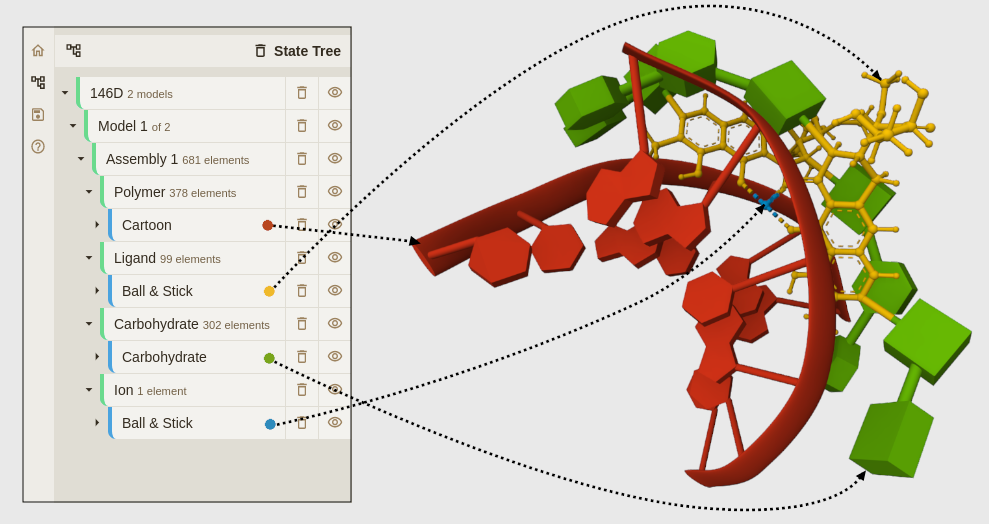
\includegraphics[width=\textwidth]{figures/state_tree.png}
  \end{center}
  \caption{Mol* state tree.}
  \label{fig:state_tree}
\end{figure}

\section{Custom mmCIF categories}
\label{section:custom_mmcif_categories}

To store partial atomic charges within a single file, we developed custom categories within the mmCIF format. The mmCIF format was chosen because it is widely used in the field of structural biology and offers several advantages over other formats, as discussed in \ref{subsection:mmcif}. The custom categories allow us to store information about the partial atomic charges separately from the other structural data, while still being able to access it within the same file. Storing all data in one file was important as it allowed for easier management and distribution of the data. If the charges were stored separately, we would have to provide the charge data to Mol* in a different way e.g. through custom import controls.


We used two separate categories for this purpose: one to store the partial charge values for each atom in the structure, and another to store metadata about the charge sets.

The category \texttt{\_sb\_ncbr\_partial\_atomic\_charges} maps together the atoms of the structure and their charges. The category has three attributes:

\begin{itemize}
  \item \texttt{type\_id} - pointer to the \\ \texttt{\_sb\_ncbr\_partial\_atomic\_charges\_meta.id} item
  \item \texttt{atom\_id} - pointer to the \texttt{\_atom\_site.id} item described in \ref{subsection:mmcif}
  \item \texttt{charge} - partial charge value for the atom
\end{itemize}

The category \texttt{\_sb\_ncbr\_partial\_atomic\_charges\_meta} is dedicated to storing metadata about the charge sets. The metadata category has the following attributes:

\begin{itemize}
  \item \texttt{id} - unique identifier for the charge set
  \item \texttt{type} - type of the calculation method (e.g. 'empirical', 'quantum')
  \item \texttt{method} - computation method used to calculate the charge set (e.g. 'EQeq', 'EEM/Racek 2016 (ccd2016\_npa)')
\end{itemize}

Figure \ref{fig:mmcif_erd} provides a detailed illustration of the custom mmCIF categories and their relationships.

\begin{figure}
  \begin{center}
    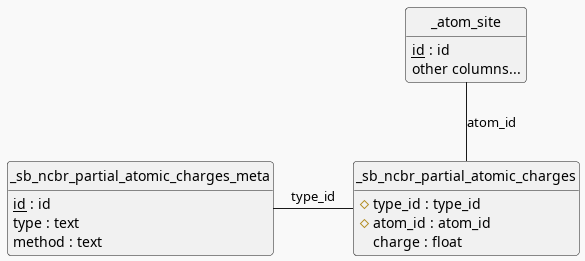
\includegraphics[width=\textwidth]{figures/mmcif_erd.png}
  \end{center}
  \caption{Diagram of custom mmCIF categories.}
  \label{fig:mmcif_erd}
\end{figure}

\section{Implementation}
\label{section:implementation}

This section will detail the implementation of the extension. The extension consists of multiple providers. Each provider serves a distinct functionality, such as supplying the partial charge data and coloring the structural elements based on their charges. The providers will be described in detail in the following subsections.

The extension was created using TypeScript, a superset of JavaScript that adds static typing and other features to the language. The Mol* library is also written in TypeScript, so the extension was written in the same language to ensure compatibility.

\subsection{Property provider}
\label{subsection:property_provider}

In order to retrieve the charges from the mmCIF file, it is necessary to parse the file. This is done by the Mol* library, which parses the mmCIF file and provides the parsed mmCIF file data in the form of a \texttt{MmcifFormat} object. The purpose of this provider is to process the charge data from this object and supply the charge data to the rest of the extension providers through a custom property. The interface of this property is depicted in Figure \ref{figure:charge_data_structure}.

The atom charges are stored in the \texttt{typeIdToAtomIdToCharge} map. The map is indexed by the charge set (typeId) and the atom id. The atom id is a pointer to the atom\_site.id. item in the mmCIF file. The atom charges are retrieved from the mmCIF file by iterating over the atom\_site.id category and retrieving the charge values for each atom. The charge values are then stored in the \texttt{typeIdToAtomIdToCharge} map.

The residue charges are calculated by summing the charges of the atoms that make up the residue. The residue charge is then stored in the \texttt{typeIdToResidueIdToCharge} map.

The maximum absolute charge values of the atoms and residues are calculated and stored in the \texttt{maxAbsoluteAtomCharges} and \texttt{maxAbsoluteResidueCharges} maps. These maps are used in the color theme provider to normalize the charges to the range of 0 to 1. Additionally, the maximum absolute charge values are used to calculate the color interpolations in the color theme provider. Additionally, the maximum absolute charge of both atoms and residues is calculated and stored in the \texttt{maxAbsoluteChargesAll} map.

Lastly, the method name used to calculate the charges of a given charge set is stored in the \texttt{typeIdToMethod} map. This map is used to display the method name in the UIs.

\begin{figure}[htbp]
  \begin{center}
    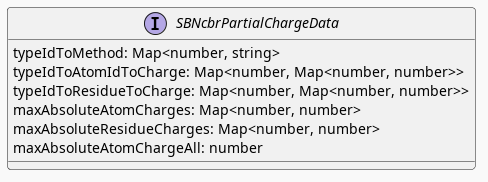
\includegraphics[width=\textwidth]{out/figures/uml/interface/custom model property interface.png}
  \end{center}
  \caption{Interface of the custom model property for storing partial atomic charges.}
  \label{fig:property_provider_interface}
\end{figure}


\begin{figure}[htbp]
  \caption{Interface of the custom model property for storing partial atomic charges.}
  \label{fig:custom_model_property}
  \definecolor{LightGray}{gray}{0.95}
  \begin{minted}[
  frame=lines,
  framesep=2mm,
  baselinestretch=1.2,
  bgcolor=LightGray,
  fontsize=\footnotesize,
  % linenos
  ]{Typescript}
    type TypeId = number;
    type IdToCharge = Map<number, number>;
    export interface SBNcbrPartialChargeData {
        typeIdToMethod: Map<TypeId, string>;
        typeIdToAtomIdToCharge: Map<TypeId, IdToCharge>;
        typeIdToResidueToCharge: Map<TypeId, IdToCharge>;
        maxAbsoluteAtomCharges: IdToCharge;
        maxAbsoluteResidueCharges: IdToCharge;
        maxAbsoluteAtomChargeAll: number;
        params: PartialChargesPropertyParams;
    }
  \end{minted}
\end{figure}

\subsection{Color theme provider}
\label{subsection:color_theme_provider}

% TODO: mention the color parameters \\

This provider serves as the central component of the extension, with its primary function being to assign colors to atoms and residues based on their charges. It achieves this by using the ColorTheme API provided by Mol*. The ColorTheme API is a mechanism for assigning colors to structural elements of a molecule. These structural elements can be atoms, residues, bonds, and so on. The API is based on the concept of a ColorTheme object, which is a collection of color assignments for structural elements. The ColorTheme object is then used by the Mol* library to color the structural elements of the molecule.

For the purposes of this extension, it was necessary to color two structural elements - atoms and residues. For both of these structural elements the charges were retrieved from the provider described in the previous section \ref{subsection:charges_provider}, which provided charges for atoms and residues.

To establish the color for a given charge, two color interpolations are employed: one for negative charges and another for positive charges. Atoms with positive charges receive a color from a white-to-blue color interpolation, while atoms with negative charges are assigned a color from a white-to-red color interpolation. These color interpolations are highlighted in Figure \ref{}. 

\begin{figure}[htbp]
  \centering
  \subfigure[Ball and stick]{\label{fig:partial_charges_color_theme-bas}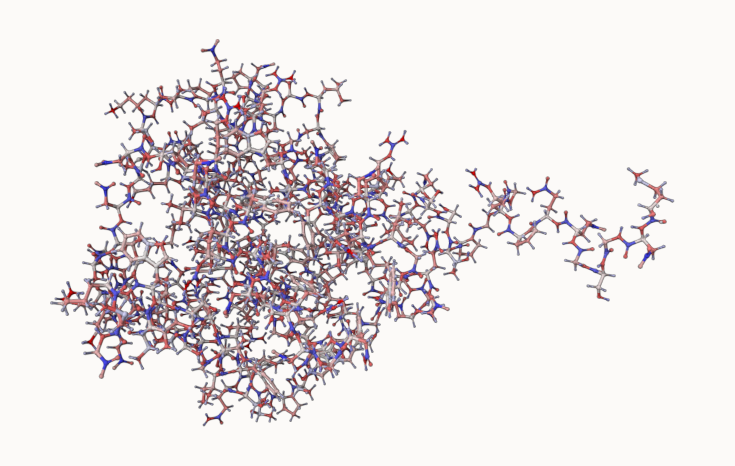
\includegraphics[width=0.45\textwidth]{figures/1F16-bas.png}}
  \subfigure[Surface]{\label{fig:partial_charges_color_theme-surface}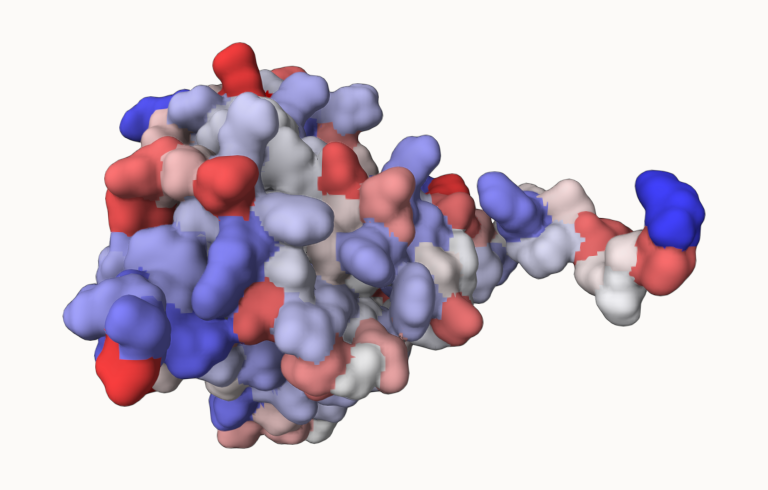
\includegraphics[width=0.45\textwidth]{figures/1F16-surface.png}}
  \subfigure[Cartoon]{\label{fig:partial_charges_color_theme-cartoon}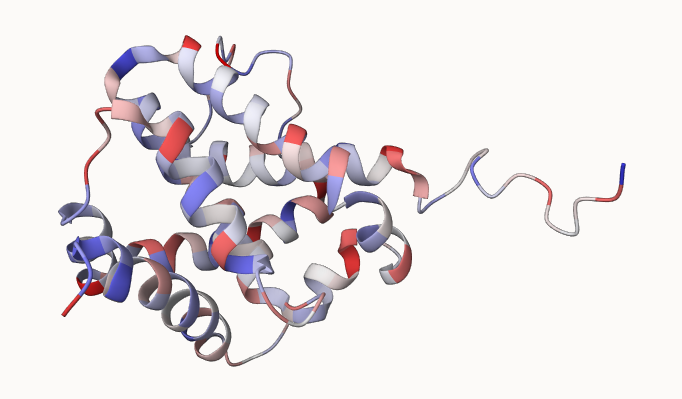
\includegraphics[width=0.45\textwidth]{figures/1F16-cartoon.png}}
  \caption{Partial charges color theme for different visualization types.}
  \label{fig:partial_charges_color_theme}
\end{figure}

\subsection{Label provider}
\label{subsection:label_provider}

% TODO: cite the Mol* documentation where the Loci object is described \\

Having colored the structural elements, it was also necessary to create a label provider, which would assign labels that describe the charge of the structural element. In order to determine which element is highlighted, Mol* uses the object Loci. A Loci object is utilized for general selections and highlights. Consequently, it is essential to first extract the location from the Loci object in order to obtain the atom ID. The charge is acquired from the property provider, and the label is an HTML string that conveys the charge of the atom or residue. An example of the label can be seen in in the right-hand corner in figure \ref{}.

\subsection{Controls}
\label{subsection:controls}

The controls are implemented automatically by the Mol* library based on the parameters of the providers. The user has access to controls of the charge set and the color theme. The charge set controls allow the user to select the charge set to display. The color theme controls allow the user to specify the following parameters:

\begin{itemize}
  \item \textbf{Charge Range}: Sets the range of the color interpolation
  \item \textbf{Use Range}: Toggles whether the range of the color interpolation is automatically calculated or manually specified.
  \item \textbf{Charge Type}: Selects whether to display the partial atomic charges or the partial residue charges.
\end{itemize}

The controls are depicted in Figure \ref{fig:controls-charge-set}.

\begin{figure}[htbp]
  \centering
  \subfigure[Charge set controls]{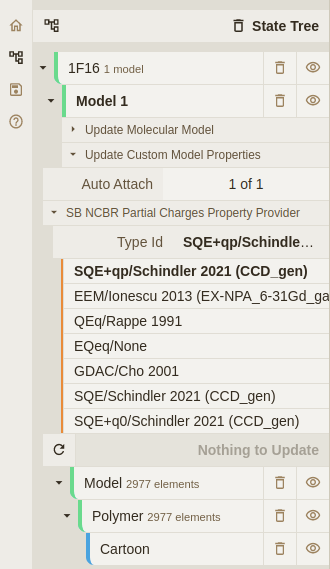
\includegraphics[width=0.49\textwidth]{figures/controls1.png}}
  \subfigure[Color theme controls]{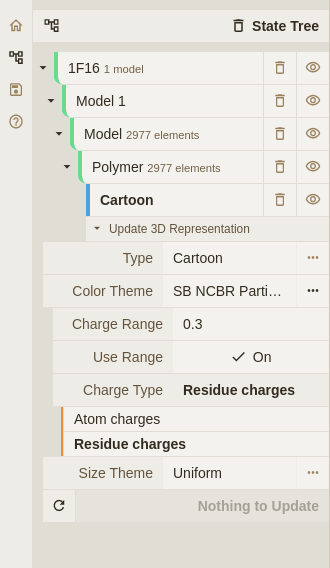
\includegraphics[width=0.49\textwidth]{figures/controls2.png}}
  \caption{Extension controls.}
  \label{fig:controls-charge-set}
\end{figure}

\section{Mol* viewer plugin}
\label{section:molstar_viewer_plugin}

In addition to the partial charges extension for the Mol* library, it was necessary to create a custom Mol* viewer plugin. By using a plugin, it is possible to create custom behavior, which is not provided by the standard Mol* viewer.

\subsection{Technologies used during development}

The plugin was developed using Vite. Vite is a build tool that was created to address some of the problems faced by developers when building large applications with traditional build tools such as Webpack. One of the main advantages of Vite is that it provides a fast development server. The speed of the development server is achieved by pre-bundling the static project dependencies with esbuild, a modern bundler written in Go, and serving the project source code with native ES module imports. \cite{vite}

The plugin is written in Typescript and uses the Mol* library. The plugin is bundled using Rollup \cite{rollup}, a module bundler for Javascript, and published to NPM, a package manager for Javascript applications. \cite{npm}

\subsection{Structure of the plugin}

The plugin is designed as a Typescript class. The structure of the class is depicted in Figure \ref{fig:plugin_structure}. It contains a method to create the plugin and another to load a structure file. Furthermore, it includes four attributes, each an object with methods that act as an interface for managing the plugin:

\begin{itemize}
  \item \textit{Charges} - provides functions for setting the charge set and retrieving information about the charge sets.
  \item \textit{Color} - provides functions for setting the color theme.
  \item \textit{Type} - provides functions for setting the visualization type.
  \item \textit{Behavior} - provides a function for focusing on a specific atom.
\end{itemize}

\begin{figure}[htbp]
  \begin{center}
    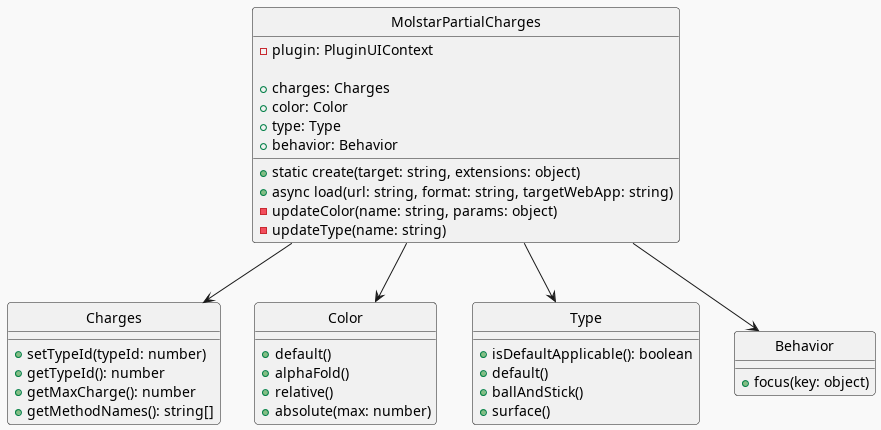
\includegraphics[width=\textwidth]{out/figures/uml/viewer/viewer.png}
  \end{center}
  \caption{Diagram of the custom Mol* viewer class.}
  \label{fig:plugin_structure}
\end{figure}

The \textit{Color} and \textit{Type} attributes set the color theme and visualization type through the private methods \textit{updateColor} and \textit{updateType}. These methods change the color theme and visualization type by iterating over the Mol* state tree and updating the representation nodes.

The focus functionality, implemented by the \textit{Behavior} attribute, is achieved by first selecting the desired atom using a query language. Mol* supports multiple query languages: MolScript, PyMOL, VMD, and Jmol. The query language used in this plugin is MolScript. The query language is used to uniquely identify and select the atom by the following attributes of the mmCIF category \textit{atom\_site}:

\begin{itemize}
  \item \textit{labelCompId} - identifier for the chain containing the residue with the atom.
  \item \textit{labelSeqId} - sequence number of the residue containing the atom.
  \item \textit{labelAtomId} - identifier for the atom in the residue.
\end{itemize}

The MolScript query selection is depicted in Figure \ref{fig:focus}. Once the atom is selected, the selection is highlighted and focused on with methods provided by the Mol* library.

\begin{figure}[htbp]
  \definecolor{LightGray}{gray}{0.95}
  \begin{minted}[
  frame=lines,
  framesep=2mm,
  baselinestretch=1.2,
  bgcolor=LightGray,
  fontsize=\footnotesize,
  % linenos
  ]{Typescript}
  const selection = Script.getStructureSelection(
    (Q) =>
        Q.struct.generator.atomGroups({
            'atom-test': Q.core.logic.and([
                Q.core.rel.eq([Q.struct.atomProperty.macromolecular.
                label_comp_id(), labelCompId]),
                Q.core.rel.eq([Q.struct.atomProperty.macromolecular.
                label_seq_id(), labelSeqId]),
                Q.core.rel.eq([Q.struct.atomProperty.macromolecular.
                label_atom_id(), labelAtomId]),
            ]),
        }),
    data
);
\end{minted}
\caption{MolScript query for selecting an atom.}
\label{fig:focus}
\end{figure}

\newpage
\chapter{Atomic Charge Calculator II}
\label{chapter:atomic_charge_calculator_ii}

Atomic Charge Calculator II (ACC~II) is a web application for calculating partial atomic charges for structure files. The application is built using Flask for the backend and Javascript with Bootstrap for the frontend. The core of the ACC~II application is the ChargeFW2 program, which is used to calculate the partial atomic charges. For visualizing the calculation results, the application uses the Litemol software. \cite{racek2020acc2} 

Since the Litemol software is no longer supported, it was necessary to replace it with its modern counterpart, Mol*. This chapter describes the incorporation of the Mol* viewer into the ACC~II application. We first discuss the modifications to the ChargeFW2 program, then explain the changes made to the backend and frontend to support calculations of multiple charge sets, and lastly we describe the integration of the Mol* viewer into the ACC~II application.

\section{Extension of ChargeFW2}
\label{section:chargefw2_extension}

As described in Section \ref{subsection:empirical_methods}, ChargeFW2 is a C++ program for computing partial atomic charges. The program supports the following input file formats: SDF, MOL2, PDB, and mmCIF, all of which are described in Section \ref{section:chemical_file_formats}. The program parses the necessary atom and bond data for each molecule in the input file and stores it in a \texttt{Molecule} object. These objects are then stored in a \texttt{MoleculeSet} object over which the program then iterates and calculates the partial atomic charges for each molecule.

The program outputs the charge results in multiple file formats. The following Table \ref{table:chargefw2_output_formats} lists the output file formats generated by ChargeFW2 for the corresponding input file formats.

\begin{table}[htbp]
  \centering
  \begin{tabular}{|l|l|}
    \hline
    \textbf{Input format} & \textbf{Output formats} \\
    \hline
    SDF, MOL2 & TXT, MOL2 \\
    \hline
    PDB & TXT, PQR \\
    \hline
    mmCIF & TXT, PQR, mmCIF \\
    \hline
  \end{tabular}
  \caption{ChargeFW2 output file formats.}
  \label{table:chargefw2_output_formats}
\end{table}

As can be seen in Table \ref{table:chargefw2_output_formats}, ChargeFW2 already outputs a mmCIF file. The format of this mmCIF file stores the partial atomic charges in a custom \texttt{\_atom\_site.fw2\_charge} item. This format, however, is not compatible with the Mol* viewer, which expects the partial atomic charges to be stored in the custom mmCIF categories described in Section \ref{section:custom_mmcif_categories}. Therefore, it was necessary to modify ChargeFW2 to output the partial atomic charges in the custom mmCIF categories.

The following subsections describe in detail how ChargeFW2 was modified to produce the custom mmCIF file format for all the input files, regardless of the input file format.

\subsection{mmCIF}

For mmCIF input files, the program simply appends the custom categories to the input file. To add the categories, the program uses the GEMMI library \cite{wojdyr2022gemmi} to parse the input mmCIF file into a \texttt{Block} object, which provides access to all mmCIF categories in the file. Before appending the charge categories, the program first removes alternative conformations from the \texttt{Block} object. This is necessary because the Mol* viewer does not support alternative conformations. The program then appends the custom charge categories to the \texttt{Block} object and writes the \texttt{Block} object to a new mmCIF file.

\subsection{PDB}

The PDB input files are first converted to mmCIF format using the GEMMI library. To achieve this, the PDB file is first parsed into a \texttt{Structure} object, which is then converted into a \texttt{Block} object. After converting the PDB file to mmCIF, it was necessary to remove the \texttt{\_chem\_comp} category from the \texttt{Block} object. This category is generated by GEMMI by default, however, it is not necessary for the Mol* viewer and its presence causes the viewer to visualize the structure incorrectly. The program then proceeds in the same way as for the mmCIF input files.

\subsection{SDF and MOL2}

Both SDF and MOL2 input files are converted to mmCIF format using the atom and bond data stored in the \texttt{Molecule} object. The program first creates a \texttt{Block} object, which it populates with the \texttt{\_atom\_site} category using the atom data. Secondly, it adds the \texttt{\_chem\_comp\_bond} category using the bond data. The later category describes the bonds between the atoms and is necessary for the Mol* viewer to visualize the bond orders correctly. The program then proceeds in the same way as for the mmCIF input files.

\subsection*{Result}

For each calculation the ChargeFW2 produces a mmCIF file, which is compatible with the Mol* viewer. The Table \ref{table:new_chargefw2_output_formats} lists the updated output file formats generated by ChargeFW2 for the corresponding input file formats.

\begin{table}[htbp]
  \centering
  \begin{tabular}{|l|l|}
    \hline
    \textbf{Input format} & \textbf{Output formats} \\
    \hline
    SDF, MOL2 & TXT, mmCIF, MOL2 \\
    \hline
    PDB, mmCIF & TXT, mmCIF, PQR \\
    \hline
  \end{tabular}
  \caption{Updated ChargeFW2 output file formats.}
  \label{table:new_chargefw2_output_formats}
\end{table}

\section{Multicharge support}
\label{section:multicharge_support}

The ACC~II application allows the user to select the method and parameters that will be used to calculate the partial atomic charges for the user's input file. Once the user confirms their selection, the application sends it to the backend, which runs the ChargeFW2 program with the chosen method and parameters. The application then displays the results of the calculation to the user.

However, the application only supports one calculation per request and does not support the visualization of multiple charge sets. This limitation was previously caused by the Litemol viewer, which only supported one charge set per structure. Since the Mol* viewer supports multiple charge sets, the ACC~II application was modified to support multiple charge sets as well.

The following subsections describe the necessary changes made to the ACC~II application to facilitate multiple calculations per one request and the visualization of multiple charge sets.

\subsection{Frontend changes}

As explained in the previous section, the ACC~II application used to limit the user to selecting only one combination of method and parameters. This limitation was resolved by introducing new controls to the calculation setup.

Figure \ref{fig:new_setup} shows the updated setup page for the ACC~II application. The page now contains a list of calculations, where each calculation represents a combination of method and parameters. The list is initially empty and the user can add a new calculation to the list by selecting the desired method and parameters from the drop-down menus and clicking the \textit{Add to calculation} button. The user can also remove any calculation from the list by clicking the cross button next to the calculation name.

Once the user clicks the \textit{Compute} button, the list of calculations is sent to the backend where it is used to generate the desired charge sets for the user's input file.

\begin{figure}[htbp]
  \begin{center}
    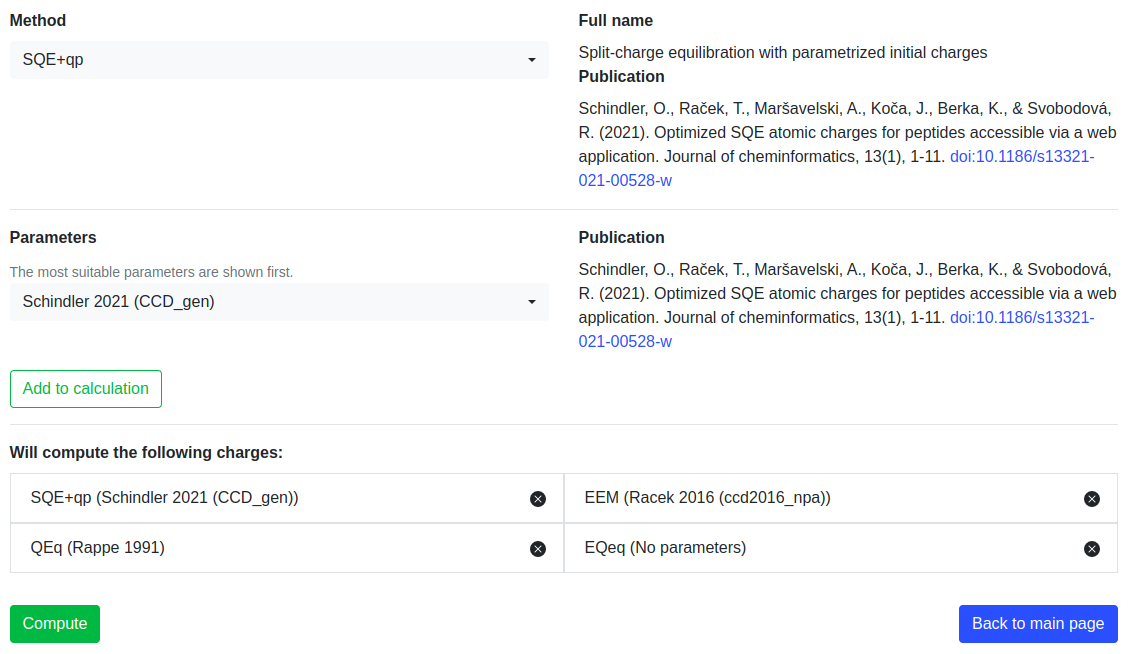
\includegraphics[width=\textwidth]{figures/new_setup.png}
  \end{center}
  \caption{Updated setup page for the ACC~II application.}
  \label{fig:new_setup}
\end{figure}

\subsection{Backend changes}

The Flask backend of the ACC~II application was modified to support multiple charge calculations per request. The backend now receives a list of calculations from the frontend, which it uses to generate the desired charge sets for the user's input file. It does this by running the ChargeFW2 program for each calculation in the list. For each calculation the ChargeFW2 generates the output file formats described in Table \ref{table:new_chargefw2_output_formats}. The backend then parses the charge values from the output TXT files and stores them in a dictionary, creating a mapping between the charge set name and the charge values.

After all of the calculations are completed, the dictionary is used to generate a single mmCIF file. Firstly, the backend parses one of the output mmCIF files generated by ChargeFW2 into a \texttt{Block} object using the GEMMI library. The backend then iterates over the dictionary and appends the charge values to the \texttt{Block} object under the custom charge categories. Lastly, the backend writes the \texttt{Block} object to a new mmCIF file. This mmCIF file is then sent to the frontend, where it is loaded into the Mol* viewer.

\section{Mol* viewer integration}
\label{section:viewer_integration}

Figure \ref{fig:result_page} shows the result page for the ACC~II application with the Mol* viewer. The result page initializes the custom viewer plugin and loads the mmCIF file generated by the backend. The loaded structure can then be visualized as a ball and stick model, as a surface model, or if applicable as a cartoon model. The page also provides controls for coloring the structure by partial atomic charges or by the element symbol of each atom. The user can also set the maximum charge value, which will be used for the partial atomic charges coloring.

The result page also contains two dropdown menus. The structure dropdown menu contains all the structures provided by the user in the input file. The charge set dropdown menu contains all the charge sets, which were generated by the backend according to the user's selection on the setup page.

\begin{figure}[htbp]
  \begin{center}
    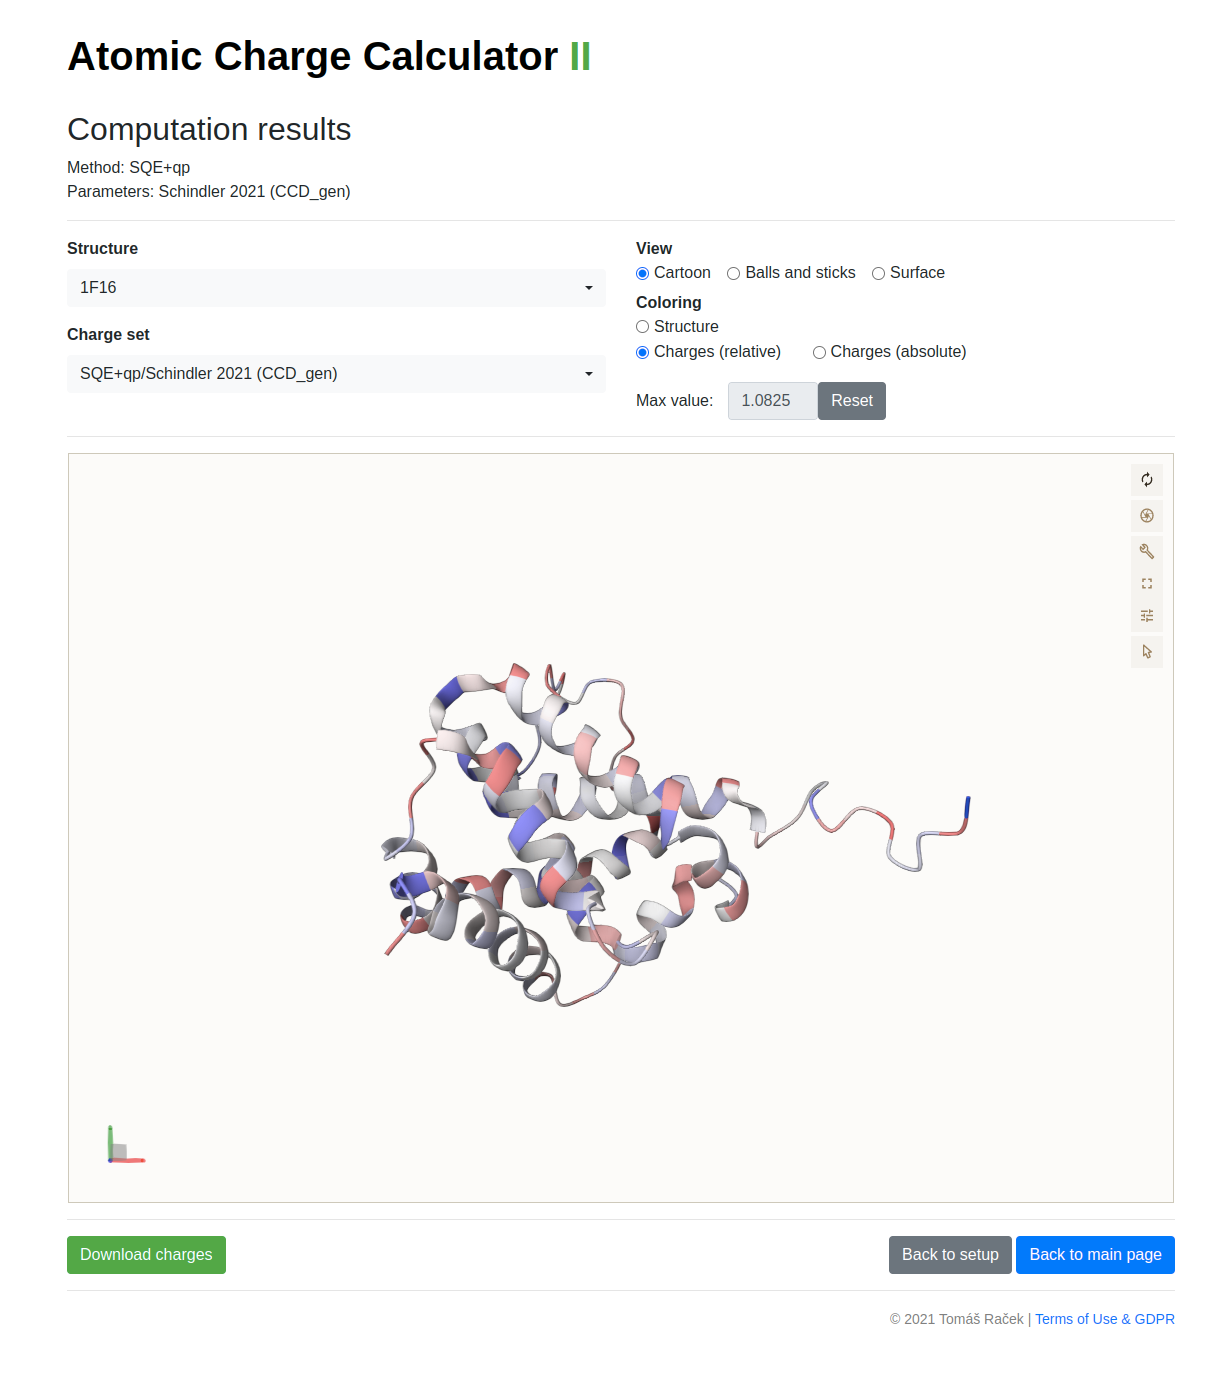
\includegraphics[width=\textwidth]{figures/results-full.png}
  \end{center}
  \caption{Updated result page for the ACC~II application.}
  \label{fig:result_page}
\end{figure}

Finally, the user can download all the output files generated by the backend in a ZIP archive by clicking the \textit{Download charges} button. Figure \ref{fig:output_dir_structure} shows the directory structure of the ZIP archive. The \texttt{cif} directory contains mmCIF files for each structure with all the charge sets. The name of each mmCIF file is the same as the name of the corresponding structure. The names of each file in the \texttt{txt}, \texttt{mol2}, and \texttt{pqr} directories are prefixed with the name of the structure and the name of the charge set (i.e. \texttt{<structure>-<parameters>.<extension>}).

\noindent
\begin{figure}[h]
  \begin{minipage}[t]{10cm}
    \dirtree{%
    .1 {charges} .
     .2 {cif} .
      .3 {1f16.fw2.cif} .
     .2 {mol2} .
     .2 {pqr} .
      .3 {1f16-EEM\_00\_NEEMP\_ccd2016\_npa.pqr} .
      .3 {1f16-SQEqp\_10\_Schindler2021\_CCD\_gen.pqr} .
     .2 {txt} .
      .3 {1f16-EEM\_00\_NEEMP\_ccd2016\_npa.txt} .
      .3 {1f16-SQEqp\_10\_Schindler2021\_CCD\_gen.txt} .
   }
   \end{minipage}\hfill
\caption{Directory structure of the output ZIP archive.}
\label{fig:output_dir_structure}
\end{figure}

\newpage
\chapter{αCharges}
\label{chapter:alphacharges}

αCharges (AlphaCharges) is a web application for calculating partial atomic charges for structures from AlphaFoldDB, a database of protein structures predicted by AlphaFold2 \cite{jumper2021alphafold}. The αCharges application protonates the protein structures (i.e. adds hydrogens) and calculates the partial atomic charges for the structures with the SQE+qp empirical method \cite{schindler2021sqe}. \cite{schindler2023alphacharges}

During the development of the αCharges application, the Mol* viewer was incorporated into the application to visualize the calculated partial atomic charges. The creators of the AlphaCharge application requested two additional features for the application: a color theme for coloring the structure by the pLDDT confidence score and a page for visualizing problematic atoms in the structure.

The following sections describe the changes made to the Mol* viewer to support the αCharges application and the implementation of the new features.

\section{Integration of the the Mol* viewer}

The αCharges application shares the architecture with the ACC~II application. The frontend is written in Javascript with the Bootstrap framework, the backend is written in Python and uses the Flask framework. This shared architecture allowed the integration of the Mol* viewer into the αCharges application with minimal adjustments. As with the ACC~II application, the Mol* viewer is incorporated into the result page by initializing the plugin viewer, loading the mmCIF file generated by the backend, and mounting the controls for managing the viewer.


\section{Coloring by pLDDT confidence score}

AlphaFold2 generates a confidence score for each residue in the predicted protein structures using a measure called pLDDT. The confidence score is a value ranging between 0 and 100, where higher values indicate higher confidence levels. \cite{varadi2021alphafold} The AlphaFoldDB includes the confidence scores along with the predicted protein structures in the mmCIF file format. These confidence scores are stored in the mmCIF file under the following categories \cite{mmcif_dictionary}:

\begin{itemize}
  \item \texttt{\_ma\_qa\_metric} - contains details of the metrics use to assess model quality.
  \item \texttt{\_ma\_qa\_metric\_local} - contains information about the local QA metrics calculated at the residue-level.
  \item \texttt{\_ma\_qa\_metric\_global} - contains information about the global QA metrics calculated at the model-level.
\end{itemize}

To incorporate this coloring into αCharges, the backend of the application was extended to include the confidence scores in the output mmCIF file. This mmCIF file is sent to the frontend where it is loaded into the Mol* viewer. The αCharges application adds a new control to the result page for switching to the pLDDT color theme. Figure \ref{fig:alpha-charges-results} shows the result page of the αCharges application and highlights the new coloring control.

\begin{figure}[htbp]
  \begin{center}
    \includegraphics[width=\textwidth,frame]{figures/alpha-charges-results.png}
  \end{center}
  \caption{Result page of the αCharges application. The control for switching to the pLDDT color theme is highlighted in red.}
  \label{fig:alpha-charges-results}
\end{figure}

\begin{figure}[htbp]
  \begin{center}
    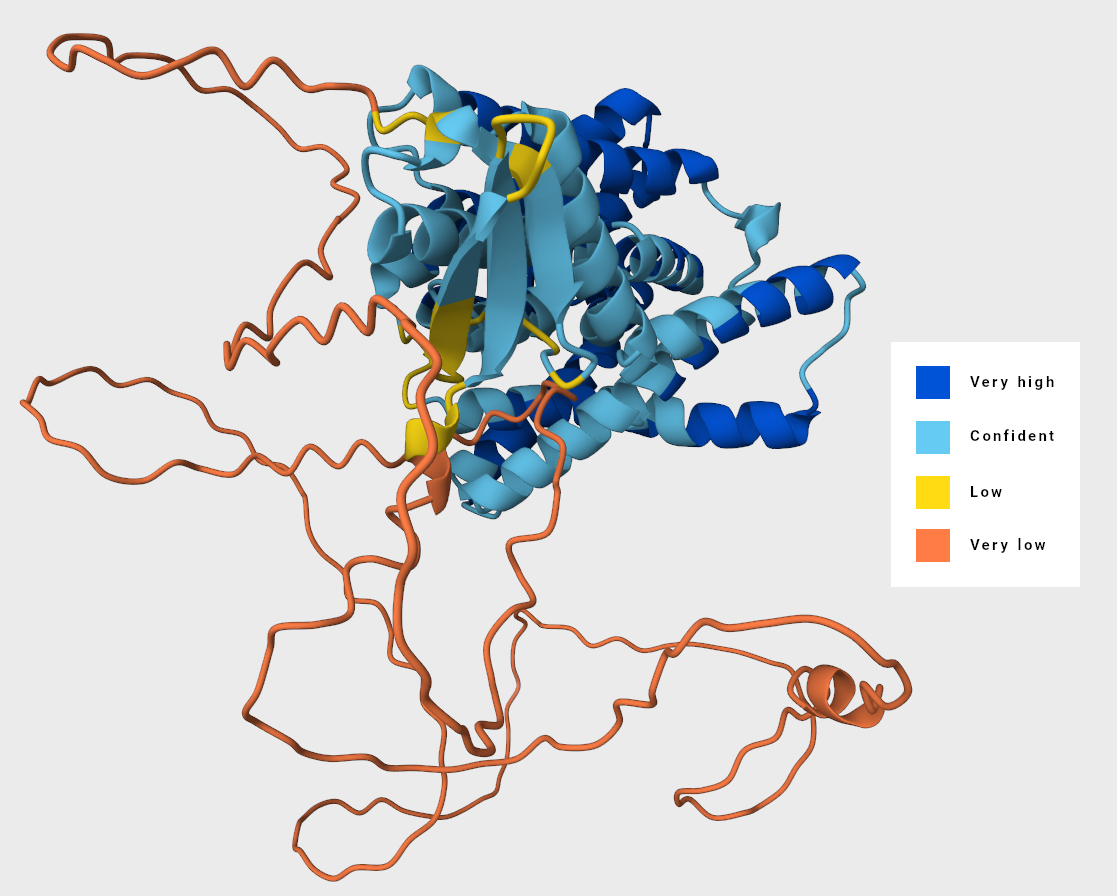
\includegraphics[width=\textwidth,frame]{figures/alphafold_coloring.png}
  \end{center}
  \caption{Coloring of the structure by the pLDDT confidence score.}
  \label{fig:alphafold-coloring}
\end{figure}

\section{Problematic structure page}

The αCharges application cannot calculate the partial atomic charges for all protein structures. Some structures can be incorrectly predicted by the AlphaFold2 algorithm or the application can fail to protonate the structure.
\cite{jumper2021alphafold} In such instances, the application automatically redirects the user to an error page, which displays the problematic structure in the Mol* viewer and an error message.

The error message is generated by the backend and contains a description of the error together with a list of each atom in the problematic structure that caused the error. When the user hovers over an atom in the list, a pop-up text is displayed with an explanation for the probable cause of the error. Figure \ref{fig:wrong_structure_text} shows the error message for a structure wrongly predicted by AlphaFold2 and the explanation for the atom \textit{GLN 33 CD}.

Additionally, when the user clicks on an atom in the list, the Mol* viewer is focused on the atom. This allows the user to inspect the atom in the structure. Figure \ref{fig:wrong_structure_focus} shows the Mol* viewer focused on the atom \textit{GLN 33 CD} of the structure Q55GB6 from AlphaFoldDB.

\begin{figure}[htbp]
  \begin{center}
    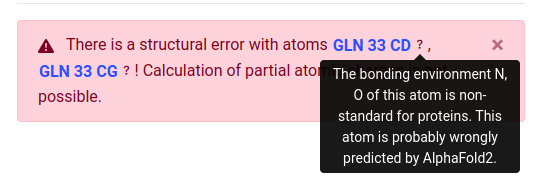
\includegraphics[width=\textwidth,frame]{figures/wrong_structure_text.png}
  \end{center}
  \caption{Explanation of error for atom \textit{GLN 33 CD}.}
  \label{fig:wrong_structure_text}
\end{figure}

\begin{figure}[htbp]
  \begin{center}
    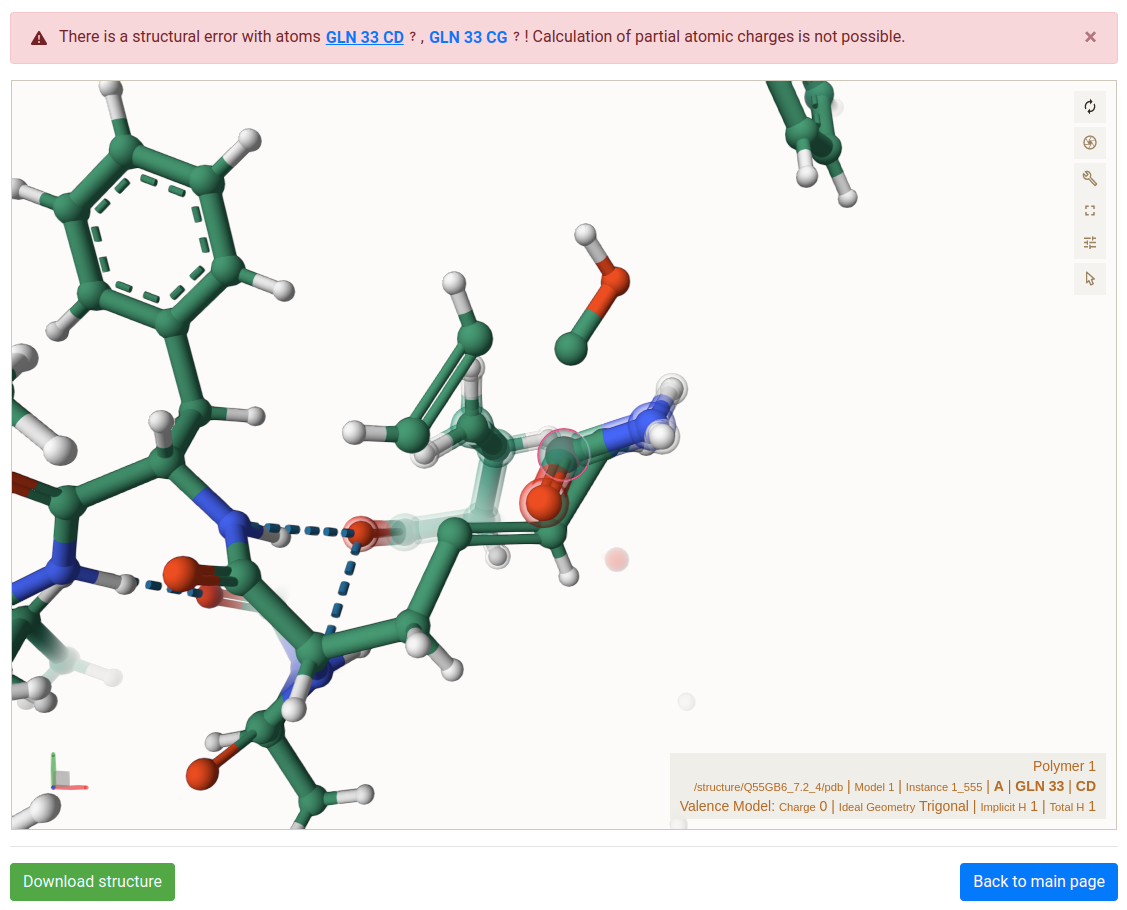
\includegraphics[width=\textwidth,frame]{figures/wrong_structure_focus.png}
  \end{center}
  \caption{Focus on the atom GLN 33 CD.}
  \label{fig:wrong_structure_focus}
\end{figure}

\newpage
\chapter*{Conclusion}
\markright{\textsc{Conclusion}}
\addcontentsline{toc}{chapter}{Conclusion}

The goal of this thesis was to extend the capabilities of the Mol* viewer to include the visualization of partial atomic charges and to incorporate the Mol* viewer into the Atomic Charge Calculator II and αCharges web applications.

We have achieved this goal by implementing a new coloring scheme for the Mol* viewer that allows the coloring of molecular structures by partial atomic charges
. Additionally, we developed an extension for the Atomic Charge Calculator II that expands the compatibility of the calculator to support multiple molecular file formats and multicharge support. The integration of the Atomic Charge Calculator II with the Mol* viewer creates a seamless workflow for analyzing and visualizing molecular structures with partial atomic charges.

In this thesis, we have explored the theory, techniques, and tools for visualizing and analyzing molecular structures with modern molecular visualization software. Our research focused on extending the capabilities of the Mol* viewer to support the visualization of partial atomic charges. 

Additionally, we have developed an extension for the Atomic Charge Calculator II that expands the compatibility of the calculator to support multiple molecular file formats and multicharge support. 

Chapter 1 laid the foundation by discussing molecular structure, partial atomic charges, chemical file formats, and color interpolation techniques. These concepts are essential for accurately representing and understanding molecular structures. By leveraging these theoretical principles, we can create informative and visually appealing visualizations.

Chapter 2 delved into various types of molecular visualizations, including ball and stick, surface, and cartoon representations. We emphasized the importance of color in visualizations to highlight specific features or properties of molecules. Additionally, we explored different visualization software, with a particular focus on the capabilities of Litemol and Mol*.

In Chapter 3, we presented the development of an extension for the Mol* viewer, specifically focusing on the incorporation of partial atomic charges. By extending the Mol* viewer, we enabled users to analyze and visualize atomic charges, providing valuable insights into the electrostatic properties of molecules. The implementation of property providers, color theme providers, label providers, and controls enhanced the user experience and facilitated the analysis of molecular structures.

Chapter 4 introduced the Atomic Charge Calculator II, an extension built upon the ChargeFW2 framework. This extension expanded the compatibility of the calculator to support multiple molecular file formats, ensuring broader accessibility for users. The integration of multicharge support further enhanced the accuracy and versatility of atomic charge calculations. The integration of the Atomic Charge Calculator II with the Mol* viewer created a seamless workflow for analyzing and visualizing molecular structures with atomic charges.

In Chapter 5, we presented the AlphaCharges tool, which introduced novel functionalities to the Mol* viewer. The integration of AlphaCharges expanded the capabilities of the viewer by enabling the visualization of pLDDT confidence scores, providing users with valuable information about the reliability of structural predictions. The introduction of the problematic structure page feature further facilitated the analysis of challenging molecular structures.

In conclusion, this thesis has contributed to the advancement of molecular visualization and analysis techniques. By extending the capabilities of the Mol* viewer, we have empowered researchers and scientists with enhanced tools to gain deeper insights into molecular structures. The integration of the Atomic Charge Calculator II and the AlphaCharges tool further strengthens the analytical capabilities of the viewer. These advancements open up new possibilities for studying molecular structures in various scientific disciplines, ranging from chemistry to biochemistry and materials science.

As technology continues to evolve, we anticipate further improvements and innovations in molecular visualization software. Future research could explore additional extensions and functionalities to address emerging challenges and enhance the analysis and understanding of complex molecular systems. By pushing the boundaries of molecular visualization, we can unlock new discoveries and advancements in scientific research.

Overall, this thesis has shed light on the significance of visualizing and analyzing molecular structures, providing researchers with powerful tools to unravel the secrets of the microscopic world and contribute to advancements in various scientific fields.

Keywords: molecular visualization, molecular structures, partial atomic charges, visualization software, Atomic Charge Calculator II, AlphaCharges, scientific research.

\printbibliography[heading=bibintoc]

\newpage
\pagenumbering{roman}
\appendix

\chapter{Source code}
\label{appendix:source-code}

All source code can be found in the attachments. Additionally, the source code can be found on GitHub. Below are the links to the GitHub repositories:

\begin{itemize}
  \item αCharges: \\
  \url{https://github.com/sb-ncbr/AlphaCharges}
  \item Atomic Charge Calculator II: \\
  \url{https://github.com/sb-ncbr/AtomicChargeCalculator2}
  \item ChargeFW2: \\
  \url{https://github.com/sb-ncbr/ChargeFW2}
  \item Mol* viewer plugin: \\
  \url{https://github.com/MergunFrimen/molstar-partial-charges}
\end{itemize}

\chapter[αCharges paper]{αCharges: partial atomic charges for AlphaFold
structures in high quality}
\label{appendix:alpha-charges}

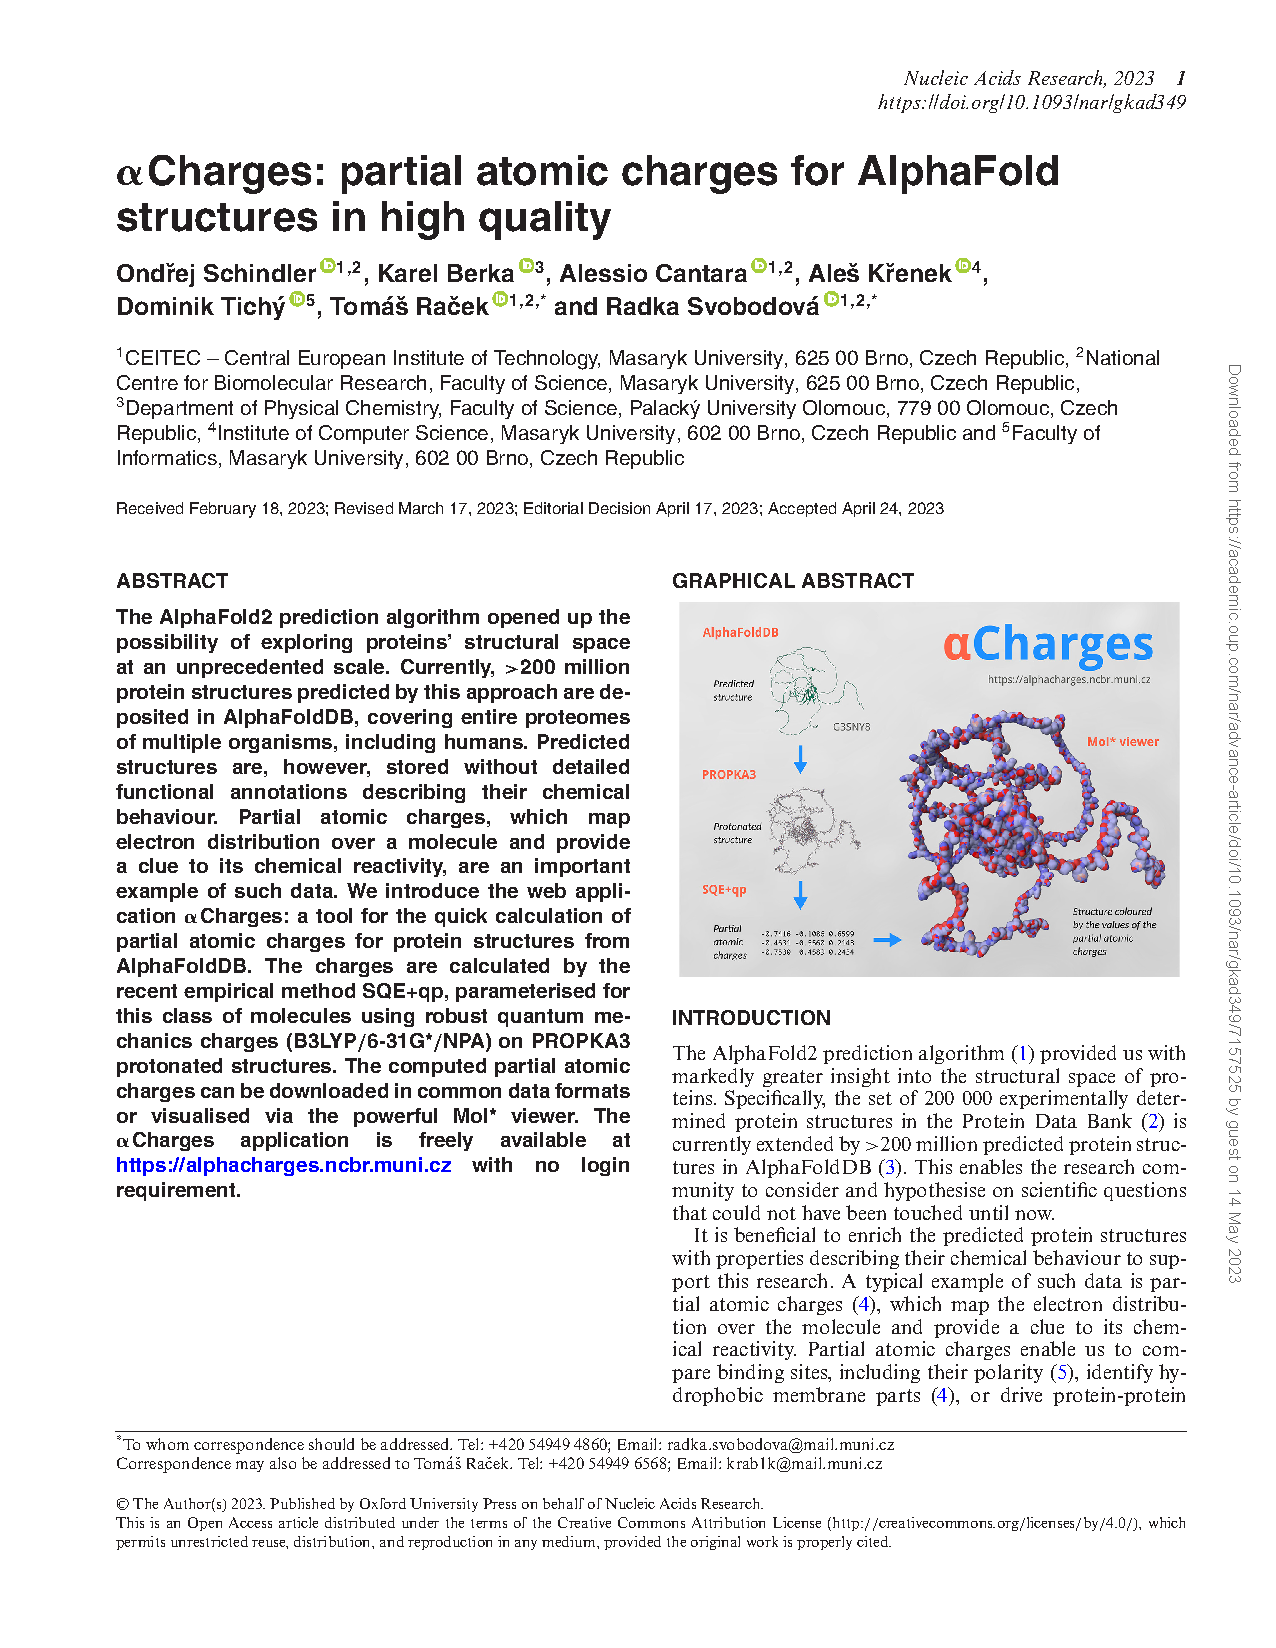
\includepdf[pages=-,width=\textwidth,offset=0cm 0cm]{figures/alphachargespaper.pdf}

\end{document}